\section{Diagramas de secuencia}

Un diagrama de secuencia muestra, en orden cronológico, los mensajes que intercambian el usuario y los componentes del sistema para realizar un caso de uso \cite{ingenieria_1}. A continuación se presentan los diagramas de los casos de uso más representativos de cada grupo: iniciar la simulación (figura \ref{fig:sequence_uc01}) y simular un paso (figura \ref{fig:sequence_uc04}), para los controles de simulación; grabar y exportar una evolución (figura \ref{fig:sequence_uc10}), para el manejo de archivos; definir la vecindad (figura \ref{fig:sequence_uc13}) y la regla de transición (figura \ref{fig:sequence_uc16}), para la configuración del autómata celular, e iniciar el entrenamiento (figura \ref{fig:sequence_uc19}), para el autómata celular neuronal. Los elementos de la interfaz se identifican con los códigos del diccionario.

\begin{figure}[H]
	\centering
	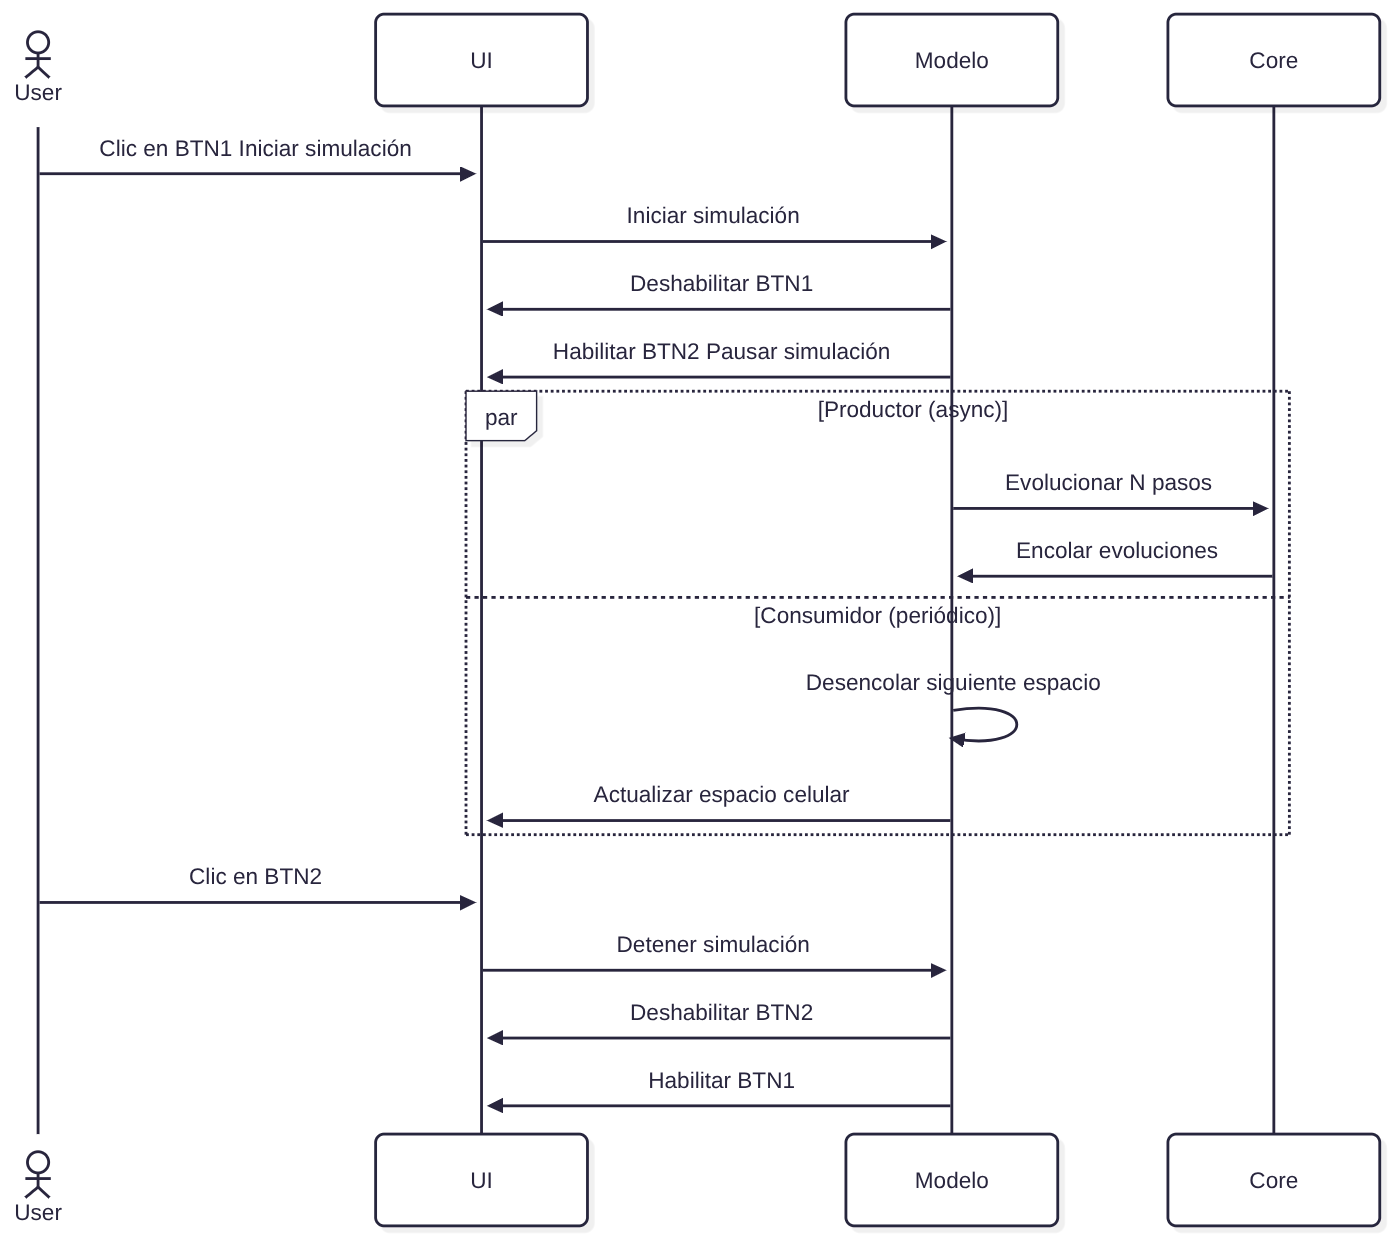
\includegraphics[width=0.95\linewidth]{img/ingenieriaSoftware/sequence_uc01.png}
	\caption{Diagrama de secuencia: UC01 Iniciar simulación.}
	\label{fig:sequence_uc01}
\end{figure}

\begin{figure}[H]
	\centering
	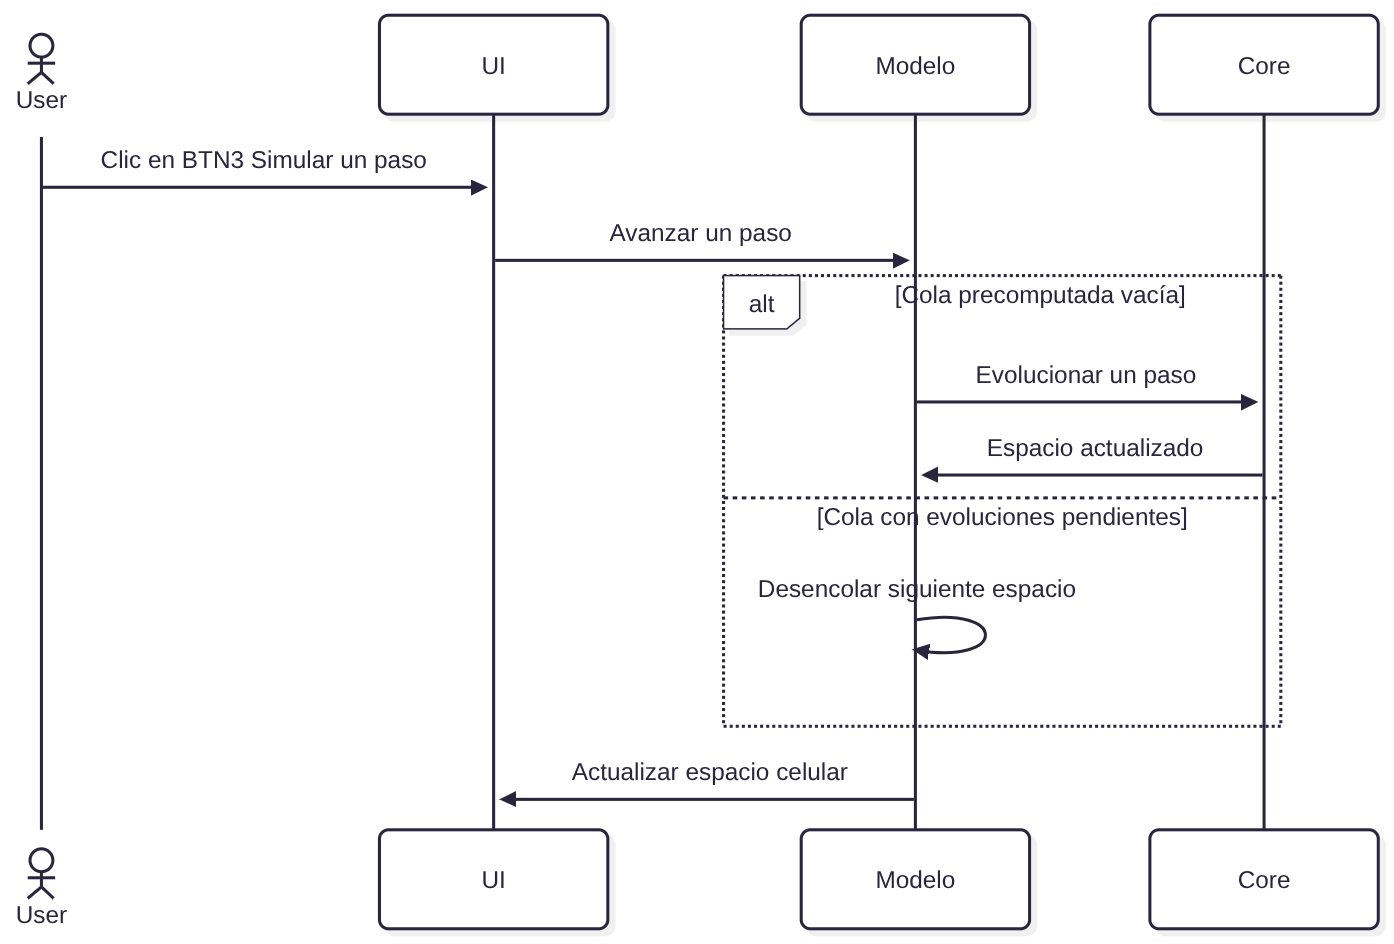
\includegraphics[width=0.95\linewidth]{img/ingenieriaSoftware/sequence_uc04.png}
	\caption{Diagrama de secuencia: UC04 Simular un paso.}
	\label{fig:sequence_uc04}
\end{figure}

\begin{figure}[H]
	\centering
	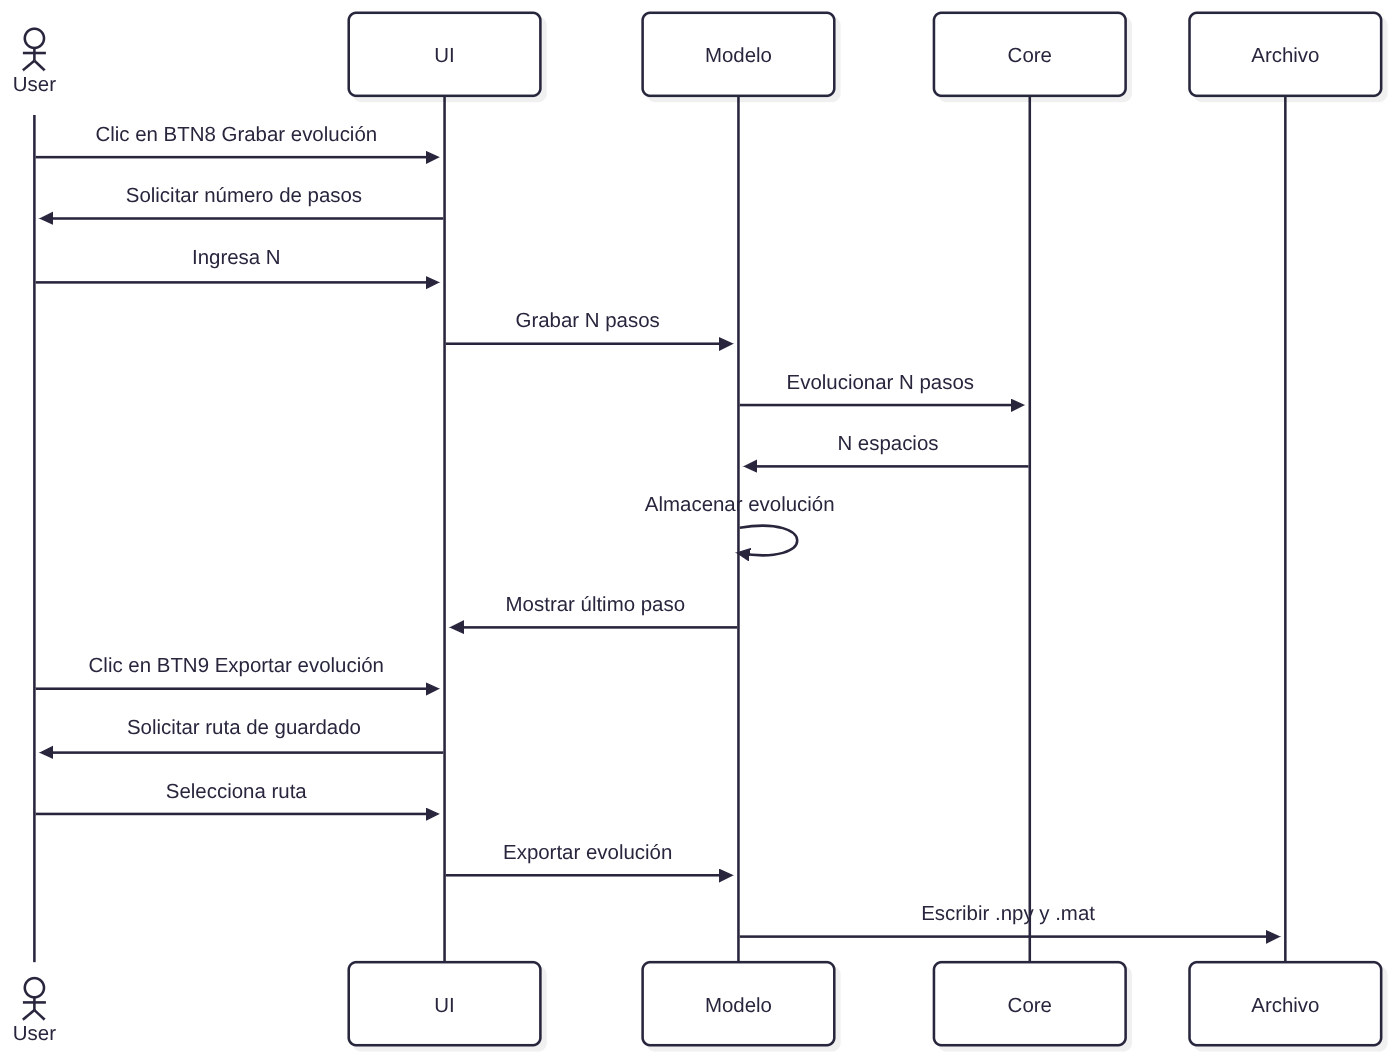
\includegraphics[width=0.95\linewidth]{img/ingenieriaSoftware/sequence_uc10.png}
	\caption{Diagrama de secuencia: UC09 Grabar evolución y UC10 Exportar evolución.}
	\label{fig:sequence_uc10}
\end{figure}

\begin{figure}[H]
	\centering
	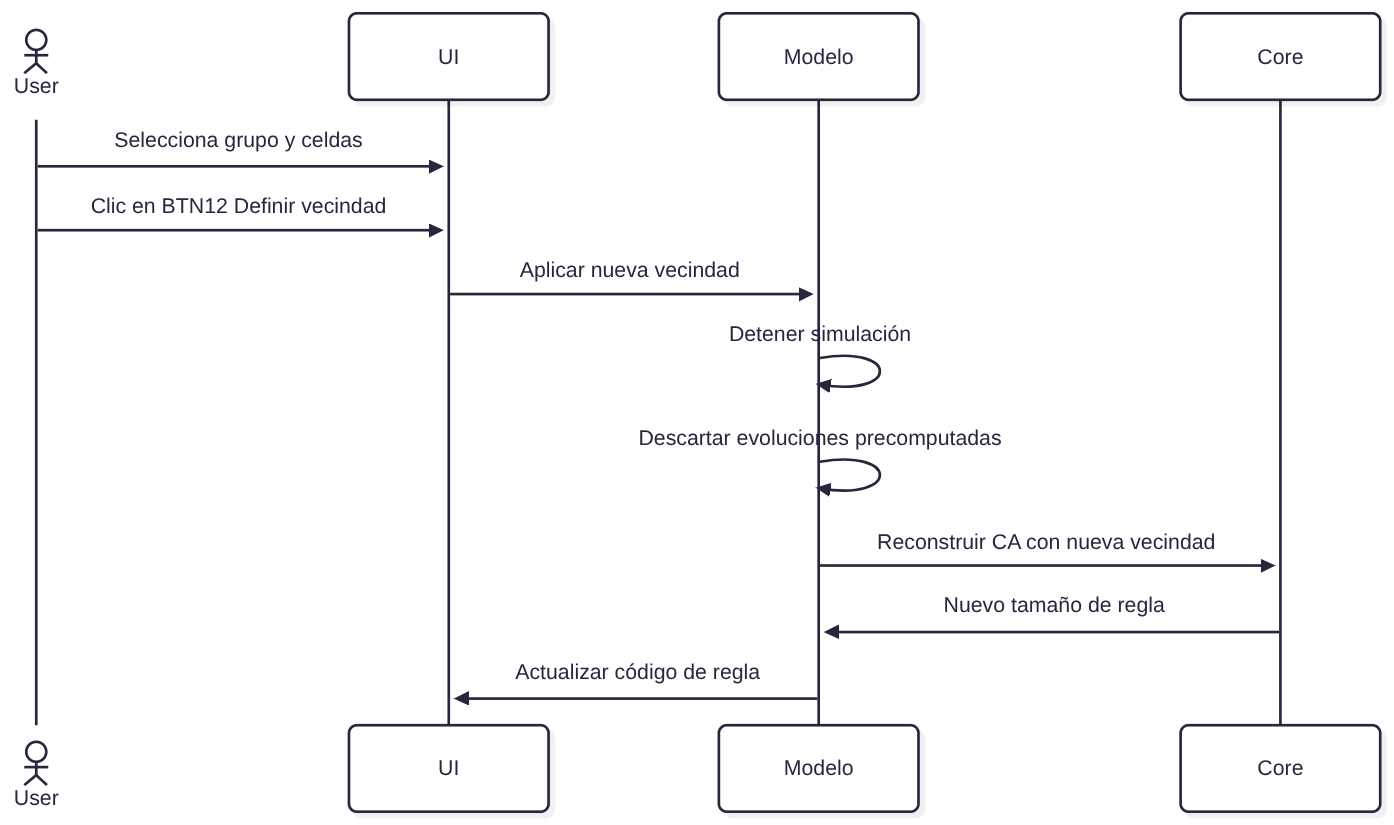
\includegraphics[width=0.95\linewidth]{img/ingenieriaSoftware/sequence_uc13.png}
	\caption{Diagrama de secuencia: UC13 Definir vecindad.}
	\label{fig:sequence_uc13}
\end{figure}

\begin{figure}[H]
	\centering
	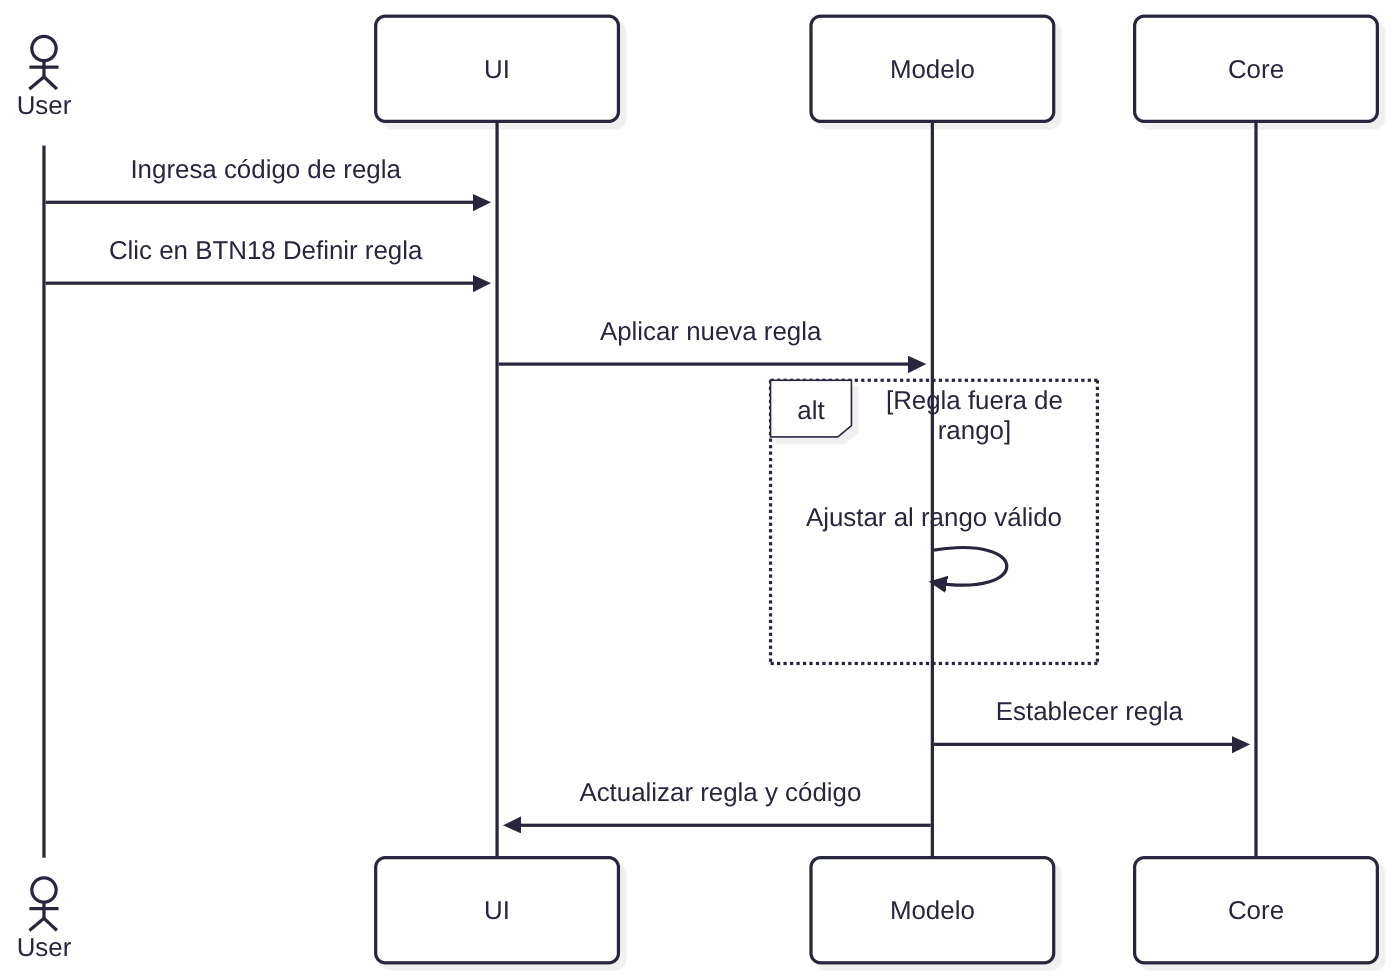
\includegraphics[width=0.95\linewidth]{img/ingenieriaSoftware/sequence_uc16.png}
	\caption{Diagrama de secuencia: UC16 Definir regla de transición.}
	\label{fig:sequence_uc16}
\end{figure}

\begin{figure}[H]
	\centering
	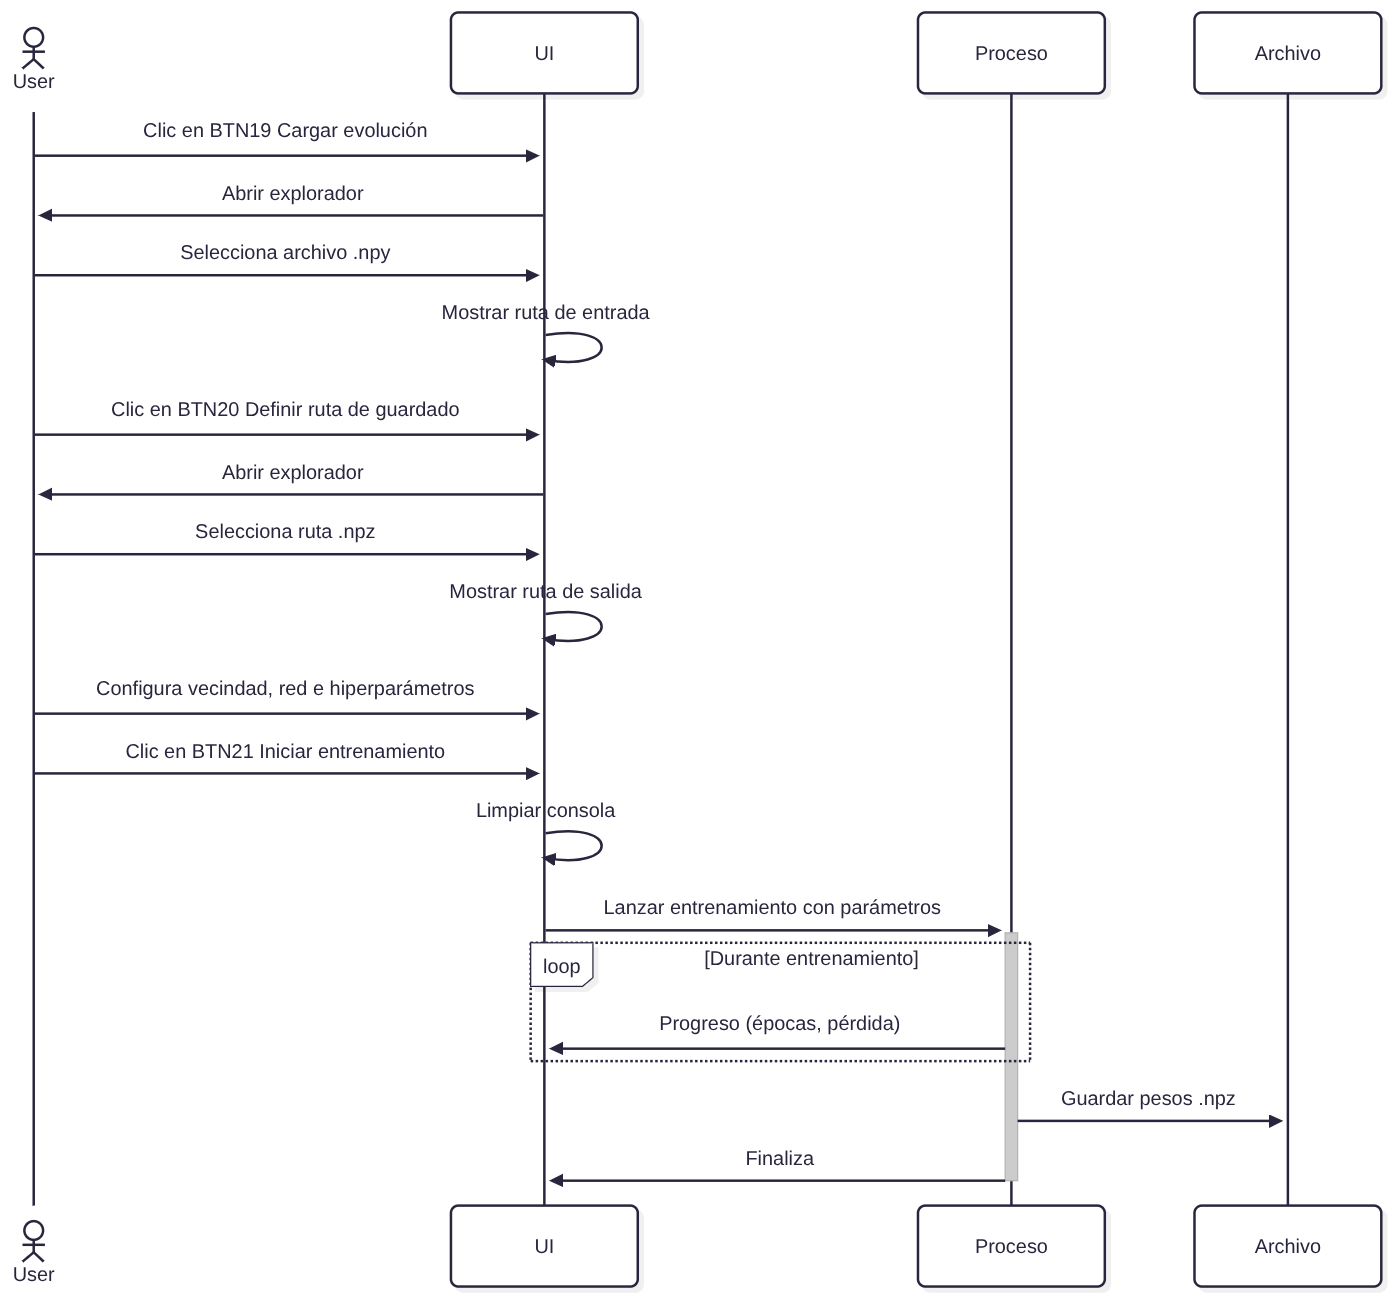
\includegraphics[width=0.95\linewidth]{img/ingenieriaSoftware/sequence_uc19.png}
	\caption{Diagrama de secuencia: UC19 Iniciar entrenamiento.}
	\label{fig:sequence_uc19}
\end{figure}

\begin{comment}
	\begin{figure}[H]
		\centering
		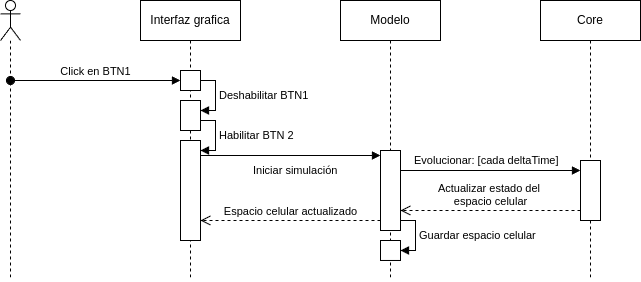
\includegraphics[width=0.9\linewidth]{img/ingenieriaSoftware/UML_SD_UC01.png}
		\caption{Diagrama de secuencia: UC01 Iniciar simulación.}
		\label{fig:UML_SD_UC01}
	\end{figure}
	
	\begin{figure}[H]
		\centering
		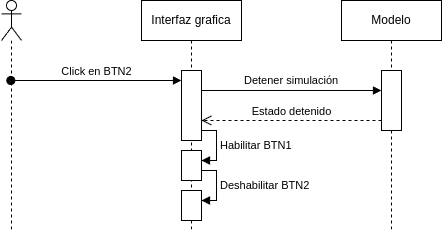
\includegraphics[width=0.7\linewidth]{img/ingenieriaSoftware/UML_SD_UC02.png}
		\caption{Diagrama de secuencia: UC02 Pausar simulación.}
		\label{fig:UML_SD_UC02}
	\end{figure}
	
	\begin{figure}[H]
		\centering
		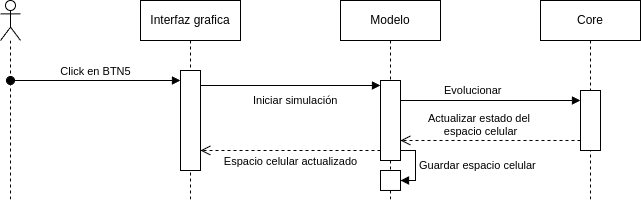
\includegraphics[width=0.9\linewidth]{img/ingenieriaSoftware/UML_SD_UC05.png}
		\caption{Diagrama de secuencia: UC05 Simular un paso.}
		\label{fig:UML_SD_UC05}
	\end{figure}
	
	\begin{figure}[H]
		\centering
		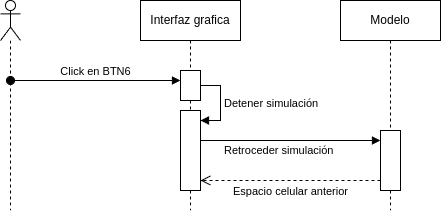
\includegraphics[width=0.7\linewidth]{img/ingenieriaSoftware/UML_SD_UC06.png}
		\caption{Diagrama de secuencia: UC06 Retroceder un paso.}
		\label{fig:UML_SD_UC06}
	\end{figure}
	
	\begin{figure}[H]
		\centering
		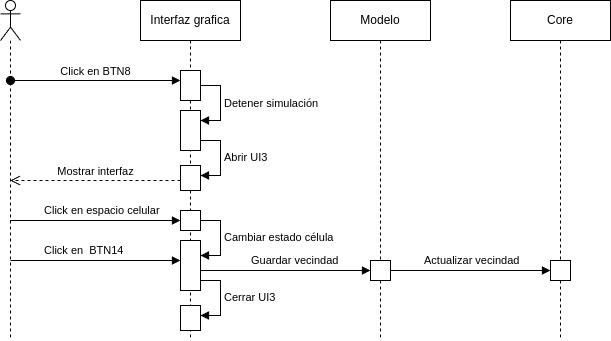
\includegraphics[width=0.9\linewidth]{img/ingenieriaSoftware/UML_SD_UC08.png}
		\caption{Diagrama de secuencia: UC08 Definir vecindad.}
		\label{fig:UML_SD_UC08}
	\end{figure}
	
	\begin{figure}[H]
		\centering
		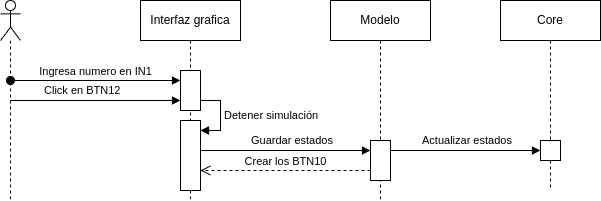
\includegraphics[width=0.9\linewidth]{img/ingenieriaSoftware/UML_SD_UC11.png}
		\caption{Diagrama de secuencia: UC11 Definir numero de estados.}
		\label{fig:UML_SD_UC11}
	\end{figure}
	
	\begin{figure}[H]
		\centering
		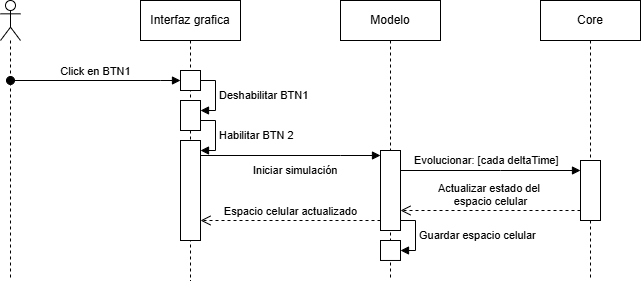
\includegraphics[width=0.9\linewidth]{img/ingenieriaSoftware/UML_SD_UC12.png}
		\caption{Diagrama de secuencia: UC12 Definir función de transición.}
		\label{fig:UML_SD_UC12}
	\end{figure}
\end{comment}


